\subsection{Algorithms}

% \begin{frame}[c,plain,noframenumbering]
% \begin{tikzpicture}[remember picture,overlay]
% \fill[fill=gray]
%     (current page.south east)  rectangle ([shift={(0,-0.1\paperheight)}]current page.north west)   ;
% \end{tikzpicture}
% \centering
% \vfill
% \textcolor{white}{\Large\textbf{Algorithms}}
% \end{frame}

\begin{frame}[fragile]{Inserting an Algorithm}
\vspace{.5cm}
	\begin{columns}[t]
		\begin{column}{.5\textwidth}
			Many packages exist to typeset an algorithm
			\\\quad\pack{algorithmic}
			\\\quad\pack{algorithm2e}
			\\\quad\pack{algpseudocode}
			\vskip.05\textheight
			Suggested: algpseudocode
		\end{column}
		\begin{column}{.5\textwidth}
			Algorithm typically embedded in an algorithm environment
			\begin{itemize}
			\item[] \pack{algorithm}
			\\\envs{algorithm}{\\\quad...\\}
			\end{itemize}
		\end{column}
	\end{columns}	
\end{frame}

\begin{frame}[fragile]{Inserting an Algorithm}
%\vspace{.5cm}
	\begin{columns}[t]
		\begin{column}{.5\textwidth}
			\begin{figure}
			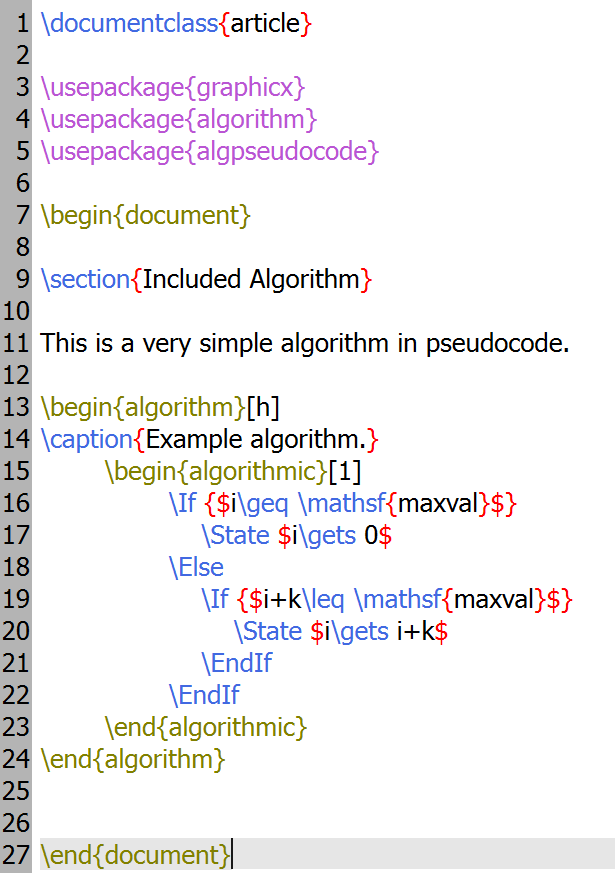
\includegraphics[scale=.4]{Figures/code5}
			\end{figure}
		\end{column}
		\begin{column}{.5\textwidth}
			\begin{figure}
			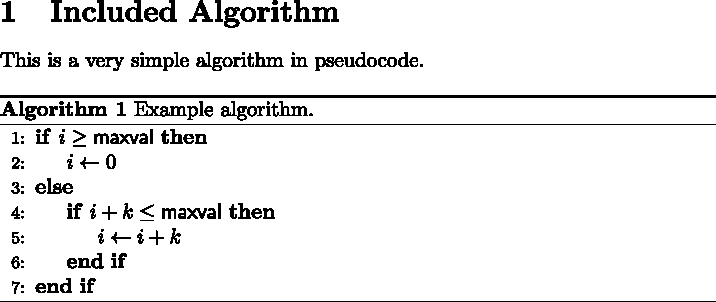
\includegraphics[width=.9\linewidth, frame, trim={-1cm -1cm -1cm -1cm},clip]{Figures/doc7}
			\end{figure}
		\end{column}
	\end{columns}	
\end{frame}

